\chapter[Magic-sets Rewrite]{Magic-sets Rewrite}
\label{ch:magic}

Having described the Evita Raced infrastructure, we now turn to the issue of
specifying query optimizations in \OVERLOG.  In this section we describe the
magic-sets rewrite compiler stage developed for Evita Raced.  Datalog-oriented
systems like P2 perform a bottom-up (\emph{forward chaining}) evaluation on
each rule, starting with known facts (tuples), and recursively deriving new
facts through rule deductions.  The advantage of this strategy is that the
evaluation is data driven (from known facts to possible deductions) and will
not enter infinite loops for some statically verifiable \emph{safe} programs.

In contrast, top-down (\emph{backward chaining}) evaluation (e.g., in the
Prolog language), starts with the query predicates as the top-level goals, and
recursively identifies rules whose head predicates unify with needed goals,
replacing them with the subgoal predicates in the rule body, until all subgoals
are satisfied by known facts or rejected when no further recursion is possible.
The advantage of a top-down evaluation strategy is that it avoids resolving
goals that are not needed by the posed queries.

\begin{figure*}[!t]
\ssp
\centering
\begin{boxedminipage}{\linewidth}
r1 {\bf path}(@X, Y, P, C) :- \\
\datalogspace {\bf link}(@X, Y, C), P := f\_cons(X, Y). \\
\\
r2 {\bf path}(@X, Y, P, C) :- \\
\datalogspace {\bf link}(@X, Z, C1), path(@Z, Y, P2, C2),\\
\datalogspace f\_contains(X, P2) == false, \\
\datalogspace P := f\_cons(X, P2), C := C1 + C2. \\
\\
Query: path(@LOCALHOST, ``localhost:10000'', P, C).
\end{boxedminipage}
\caption{\label{ch:evita:fig:querySP}Relevant rules copied from Figure~\ref{ch:p2:fig:overlogSP}.}
\end{figure*}

The magic-sets technique rewrites logical rules so that bottom-up evaluation
over the rewritten rules has all advantages of top-down and bottom-up
evaluation strategies.  We review those advantages here by example using the
shortest path program shown in Figure~\ref{ch:evita:fig:querySP}.  A
straightforward bottom-up evaluation of this program applies the \ol{link}
tuples to rule \ol{r1}, creating the initial {\tt path} tuples.  Rule \ol{r2}
derives all \ol{path} tuples, while any \ol{path} tuples matching
``localhost:10000'' on their second attribute are returned by the programmer's
query.

The bottom-up evaluation generates some \ol{path} tuples that do not have
``localhost:10000'' in the second attribute and therefore cannot satisfy the
programmer's query.  In contrast, a top-down evaluation begins by unifying the
query predicate with the head predicate of rules \ol{r1} and \ol{r2}.
Therefore, the \ol{path} predicate unification binds the $@X$ attribute to the
current node identifier and the $Y$ attribute to ``localhost:10000'' in both
rules, which is carried over to the predicates in the rule body.  The binding
of $@X$ and $Y$ attributes in rules \ol{r1} and \ol{r2} means that these rules
will only look for tuples of the form
\ol{path(``127.0.0.1'', ``localhost:10000'', P, C)} as well as tuples that can help
form such \ol{path} tuples, but nothing else.

In Section~\ref{ch:magic:sec:background} we review the literature

\section{Background}

The magic-sets rewrite is an optimization that can reduce the amount of
computation in recursive Datalog queries by deriving only those tuples that are
relevant to query predicates posed by a program.  It does this by adding extra
selection predicates to the rules of a program to emulate the goal-oriented
execution of top-down evaluation (his is sometimes called \emph{sideways
information passing} or SIP).  Conceptually, given a rule of the form \[ H_p
\text{\ol{:-}}\ G_1, G_2, ..., G_k \] where $H_p$ is the head predicate $p$ and
$G_{1,...,k}$ are the goal predicates in the order of appearance in the rule, a
magic-sets algorithm intersperses selection predicates $s_{1,...,k}$ to
generate rule $H_p \ \text{\ol{:-}}\ s_1, G_1, s_2, G_2, ..., s_{k}, G_k$.
Facts for these selection predicates are generated according to bindings of
attributes, in the user's query or other rule predicates in the program, to
constant values.

Before we present the declarative rules for implementing this rewrite
technique, we review the concept of adornments and the ``rule/goal graph''
representation for a collection of \OVERLOG (Datalog) rules.  These data
structures form the basis of the magic-sets algorithm, and hence our
declarative rules for it.


\subsection{Adornments}

Consider again a snippet of the shortest path program in Figure~\ref{ch:evita:fig:querySP}.  
The query predicate \ol{path(@LOCALHOST,
``localhost:10000'', P, C)} asks for the shortest path from all nodes to node
``localhost:10000''.  We can indicate which path arguments are bound and which
are free by an {\emph adornment}, which is a binding pattern that contains a
string of {\emph b's} and {\emph f's} of length {\emph k}, for each {\emph k}
arguments of path.  In the current context, the {\emph path} query predicate has
a $path^{ffbb}$ adornment since the first two arguments are bound to constants
and the last two are free variables.

Each rule in an \OVERLOG program is also given an adornment according its
evaluation based on the sideways information passing algorithm described in
Section~\ref{ch:intro}.  The steps for assigning rule adornments are as
follows.
\begin{enumerate}
\item A variable appearing in a bound argument of the rule head is bound before processing any subgoals.
\item A variable is bound after processing subgoal $G_i$ if it was bound
  before processing $G_i$ or if it appears anywhere in $G_i$.
\end{enumerate}
The format of a rule adornment differs from a predicate.  It follows the form
$[X_1,\cdots,X_m|Y_1,\cdots,Y_n]$, which contains two sublists of variables
separated by a bar.  The variables to the left of the bar (i.e.,
$X_1,\cdots,X_m$) represent bound variables, while those to the right (i.e.,
$Y_1,\cdots,Y_n$) are free. 

A given rule contains a number of these binding patterns, one for each subgoal
position.  A rule adornment is a binding pattern of a rule at a particular
position.  The notation that we follow for rule adornments identifies rule
positions as a subscript and binding patterns as a superscript.  For example,
$r1_0^{[X,Y|P,C]}$ is the adornment for rule \ol{r1} at position $0$, which
takes on the binding pattern of the head predicate relative to the
$path^{bbff}$ adornment. Continuing, $r1_1^{[X,Y,C|P]}$ represents the rule
adornment at position $1$, following the \ol{link} predicate, which adds
$C$ to the list of bound variables. Finally, $r1_2^{[X,Y,C,P]}$ is the
rule adornment following the assignment, and therefore binding, of the variable
$P$.

\subsection{Rule/Goal Graphs}

\begin{figure*}[!t]
\begin{center}
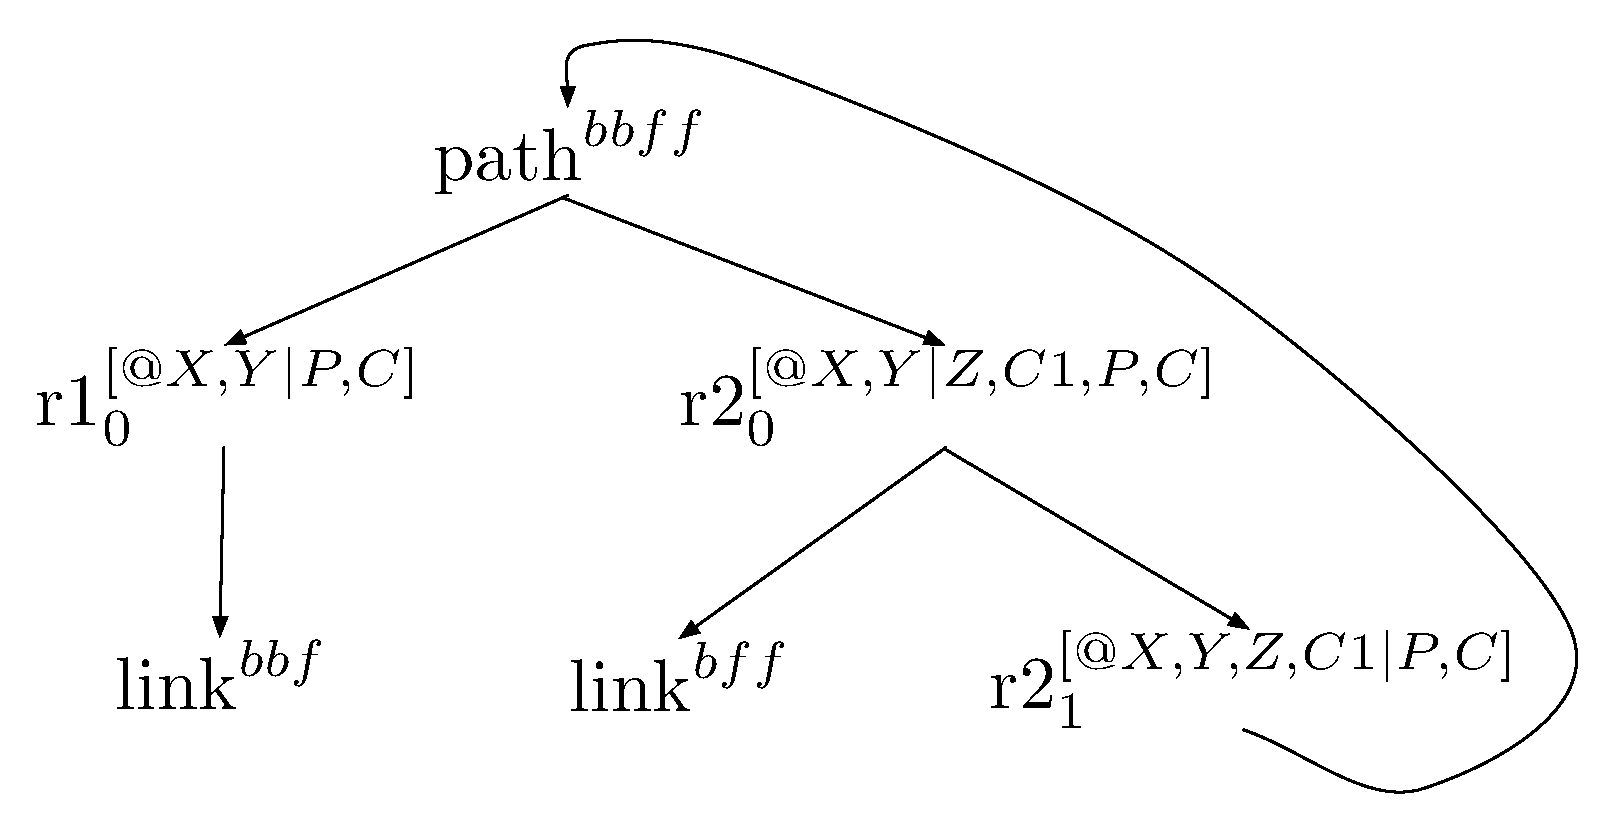
\includegraphics[scale=1.8]{figures/RuleGoalGraph}
\caption{Rule/Goal graph of the program in Figure~\ref{ch:evita:fig:querySP}.}
\label{ch:evita:fig:rggraph}
\end{center}
\end{figure*}

A rule/goal graph is a representation of binding patterns that occurs in a
collection of rules.  The graph consists of \emph{rule} and \emph{goal}
vertices.  A goal vertex consists of a predicate with an adornment, and
similarly, a rule vertex represents the adornment of the rule in a particular
position accoring to its left-to-right execution.

Figure~\ref{ch:evita:fig:rggraph} illustrates the full {\em Rule/Goal} graph
for our shortest path example.  To build this graph, the algorithm starts with
a goal predicate (at first, this is the query predicate---\ol{path} in our
example), and creates a goal vertex in the graph with the appropriate adornment
($\mathit{bbff}$ for \ol{path} since the query binds its first two variables to
constant values).  For every rule with that goal predicate as its head, the
algorithm traverses the rule body from left to right, creating a child rule
vertex for every $0$-th position variable binding.  For rule \ol{r2} in the
example, the rule vertex for position $0$ ($r2_0$) has variable state
$[X,Y|P,C]$, which denotes that variables \ol{X,Y} are bound (to the same
values as those ``pushed down'' from the goal vertex) and \ol{P,C} are free.
Given a rule vertex for position $i$, two children are created: a goal vertex
for the next predicate after position $i$ and a rule vertex for the next
position in the rule (unless the body's end has been reached).  In the running
example, the child goal vertex corresponds to the {\tt link} predicate that
appears at position $0$, with adornment $\mathit{bff}$ since \ol{X} is already
bound at this point in the evaluation, but \ol{Z} and \ol{C1} are not.
Similarly, the child rule vertex at position $1$ contains the variable
signature $[X,Y,Z,C1|P,C]$ since \ol{link} added some bound variables.  

The process continues until all rule and goal vertices have been constructed
and connected; only a single goal vertex can exist with the same predicate and
adornment, as is the case for the \ol{path} vertex with adornment
$\mathit{bbff}$.  It is easy to see how the rest of the rule/goal graph is
constructed.  After all vertices have been generated given the chosen rules,
any predicates with a unique adornment in the graph are added to the goals, and
the rules producing them are recursively traversed.

\section{Declarative Magic-sets}
\label{ch:magic:sec:rules}

In Evita Raced we created a magic-sets rewrite stage written in \OVERLOG.  The
\OVERLOG rules are based on the description of the magic-sets algorithm given
in Ullman's course notes~\cite{ullmanNotes}, which begins by constructing a
rule/goal graph on the target program.  It uses the constructed rule/goal graph
to check for the {\emph unique binding property} with respect to the adornment
of the query predicate.  This property is met for query predicate $p$ {\emph
iff} the rule/goal graph contains a unique ``binding pattern'' for $p$.  The
original query predicate for $p$ provides the first binding patterns, while
rules that mention $p$ provide further bindings.  We check for this property
during our construction of the rule/goal graph.

The magic-sets rewrite involves a number of steps, which we have subdivided
into to logical groups. The first group presented in Section~\ref{ch:magic:sec:rgconstruct}
deals with the construction of the rule/goal graph for the target program.
The Metacompiler Catalog already provides some of this information through
goal (head predicate) and subgoal (body terms) rule dependencies. The remaining
information that we need to derive include the adornment information for goal and
rule nodes. Once this information is recursively obtained, we can move on to
the actual rewrite rules described in Section~\ref{ch:magic:sec:rewrite}, where
magic and supplementary relations are materialized in the target program.

\subsection{Rule/Goal Graph Construction}
\label{ch:magic:sec:rgconstruct}

The algorithm for constructing a rule/goal graph begins with the query
predicate, and recursively through the rules that mention the query predicate
in the head.  We assume the unique binding property holds in the beginning, and
detect if it does not along the way.  Techniques exists for rewriting a program
so that the unique binding property always holds but we did not consider those
in this work.  Given a query predicate $p$, we assign a {\emph magic predicate}
denoted as $m_p$ with a corresponding adornment.  A set of {\emph supplementary
predicates}, denoted as $sup_i$ ($i$ is a rule position), are also created as
we recursively walk the rules in a left-to-right (SIP) order.


\begin{figure*}[!t]
\ssp
\centering
\begin{boxedminipage}{\linewidth}

/* Create an adornment for the query predicate and add a fact to the \\
\ol{magicPred} table referencing this adornment. */ \\
ms1 {\bf magicPred}(@A, Pid, Name, Sig) :- \\
\datalogspace {\bf magic::programEvent}(@A, Pid, ...), \\
\datalogspace {\bf sys::rule}(@A, Rid, Pid, ... , Goals), \\
\datalogspace {\bf sys::predicate}(@A, \_, Rid, ..., Schema), \\
\datalogspace $Goals == 1$, \\
\datalogspace Sig := f\_adornment(Schema).
	
\end{boxedminipage}
\caption{\label{ch:magic:fig:magic1}Construction of the query adornment and corresponding magic predicate.}
\end{figure*}

Our rule in Figure~\ref{ch:magic:fig:magic1} creates an adornment for the query
predicate and adds such a fact to the \ol{magicPred} relation.  A query
predicate is identified in P2 by a rule containing a single goal ($Goals ==
1$).  The sole predicate in this rule has a schema ($Schema$) that contains
some number of (binding) constants and (free) variables.  The function {\emph
f\_adornment} takes a schema object as argument and returns a string containing
the adornment signature.

\begin{figure*}[!t]
\ssp
\centering
\begin{boxedminipage}{\linewidth}
/* Initialize sup position 0 for rules that reference a magic predicate in the head. */ \\
ms2 {\bf sup}(@A, Pid, Rid, Pos, SupName, Schema, f\_idgen()) :- \\
\datalogspace {\bf magicPred}(@A, Pid, Name, Sig), \\
\datalogspace {\bf sys::rule}(@A, Rid, Pid, RName, HeadPid, ...), \\
\datalogspace {\bf sys::predicate}(@A, HeadPid, Rid, \_, Name, ..., FSchema, ...), \\
\datalogspace Schema := f\_project(Sig, FSchema), \\
\datalogspace SupName := "sup\_" + RName + 0, \\
\datalogspace Pos := 0. \\

/* Move the rule position forward when update occurs to sup. */ \\
ms3 {\bf supNext}(@A, Pid, Rid, Pos+1, Schema) :- \\
\datalogspace {\bf sup}(@A, Pid, Rid, Pos, Name, Schema, Tid). \\
	
/* Create supplementary predicate for a given subgoal. */ \\
ms4 {\bf sup}(@A, Pid, Rid, Pos, SupName, NewSchema, f\_idgen()) :- \\
\datalogspace {\bf supNext}(@A, Pid, Rid, Pos, Schema), \\
\datalogspace {\bf sys::rule}(@A, Rid, Pid, RName, ...), \\
\datalogspace {\bf sys::predicate}(@A, Fid, Rid, ..., FSchema, Pos, ...), \\
\datalogspace SupName := "sup\_" + RName + "\_" + Pos, \\
\datalogspace NewSchema := f\_merge(Schema, FSchema). \\
	
/* Create supplementary predicate for a given assignment. */ \\
ms5 {\bf sup}(@A, Pid, Rid, Pos, SupName, NewSchema, f\_idgen()) :- \\
\datalogspace {\bf supNext}(@A, Pid, Rid, Pos, Schema), \\
\datalogspace {\bf sys::rule}(@A, Rid, Pid, RName, ...), \\
\datalogspace {\bf sys::assign}(@A, Aid, Rid, Var, \_, Pos), \\
\datalogspace SupName := "sup\_" + RName + "\_" + Pos, \\
\datalogspace NewSchema := f\_assignschema(Schema, Var). \\ 
	
/* Move supNext forward for selection predicates. */ \\
ms6 {\bf supNext}(@A, Pid, Rid, Pos+1, Schema) :- \\
\datalogspace {\bf supNext}(@A, Pid, Rid, Pos, Schema), \\
\datalogspace {\bf sys::rule}(@A, Rid, Pid, ..., Goals), \\
\datalogspace {\bf sys::select}(@A, Sid, Rid, \_, Pos, \_), \\
\datalogspace $Pos < Goals$. 
\end{boxedminipage}
\caption{\label{ch:magic:fig:magic2}Rules for supplementary relational predicates.}
\end{figure*}

The previous rule (\ol{ms1}) created the top-level goal node, which is the root
of the rule/goal graph.  The group of rules in Figure~\ref{ch:magic:fig:magic2}
deal with creating adornments for rules in the target program.  We store the
rule adornment in a \ol{sup} relation since this information will be used to
create supplementary predicates in Section~\ref{ch:magic:sec:rewrite}.  A
\ol{sup} tuple contains the following attributes in order:
\begin{itemize}
   \ssp
  \item A reference to the target program and rule identifiers. 
  \item The position within that target rule.
  \item A name for the supplementary predicate.
  \item A schema object containing all constants and variables up to that rule position.
  \item A new identifier that will be used (in Section~\ref{ch:magic:sec:rewrite}) to create 
    a new rule that supplies facts to the supplementary relation.
\end{itemize}

We now describe the details of each rule in Figure~\ref{ch:magic:fig:magic2}.
Rule~\ol{ms2} initiates the first \ol{sup} deduction.  It joins \ol{magicPred}
with the \ol{rule} and \ol{predicate} relations to obtain those rules that
contain the magic predicate in the head.  This deduction represents the
supplementary predicate in position~$0$.  The adornment for this rule position
is obtained by projecting the head predicate schema onto the magic predicate
adornment.  The function {\emph f\_project} takes the head predicate schema and
the signature of the magic predicate adornment, and return a new schema that
contains the bound head variables (according to the adornment). For example,
if the head predicate schema is $[A, B, C]$ and the adornment is $fbf$ then
the {\emph f\_project} would return $[B]$ as the new schema. This new schema
will be the schema for the current supplementary predicate.


\begin{figure*}[!t]
\ssp
\centering
\begin{boxedminipage}{\linewidth}
/* We've encountered a magic predicate in the body of a rule. \\
   Compute its adornment based on current bound variables. */ \\
ms7 {\bf magicPred}(@A, Pid, FName, Sig) :- \\
\datalogspace {\bf supNext}(@A, Pid, Rid, Pos, Schema), \\
\datalogspace {\bf sys::rule}(@A, Rid, Pid, RName, ...), \\
\datalogspace {\bf sys::predicate}(@A, Fid, Rid, \_, FName, ..., FSchema, Pos, ...), \\
\datalogspace {\bf magicPred}(@A, Pid, FName, Sig), \\
\datalogspace Sig := f\_adornment(Schema, FSchema).

\end{boxedminipage}
\caption{\label{ch:evita:fig:mpgoal}Encountering a magic predicate during subgoal traversal.}
\end{figure*}

\begin{figure*}[!t]
\ssp
\centering
\begin{boxedminipage}{\linewidth}
/* Indicate when a rule has been fully explored. */ \\
ms9 {\bf ruleComplete}(@A, Pid, Rid) :- \\
\datalogspace {\bf supNext}(@A, Pid, Rid, Pos, \_), \\
\datalogspace {\bf sys::rule}(@A, Rid, Pid, ..., Goals), \\
\datalogspace Pos >= Goals. \\
	       
/* Count the number of completed rules. */ \\
ms10 {\bf rulesComplete}(@A, Pid, a\_count<Rid>) :- \\
\datalogspace {\bf ruleComplete}(@A, Pid, Rid). \\
	        
/* Count the number of rules in a program. */ \\
ms11 {\bf programRuleCount}(@A, Pid, a\_count<Rid>) :- \\
\datalogspace {\bf programEvent}(@A, Pid, ...), \\
\datalogspace {\bf sys::rule}(@A, Rid, Pid, ...). \\
	
/* Count the number of adornments for a given magic predicate. */ \\
ms12 {\bf countAdornments}(@A, Pid, Name, a\_count<Sig>) :- \\
\datalogspace {\bf magicPred}(@A, Pid, Name, Sig). \\
	       
/* Commit a magic predicate iff it has a unique adornment. */ \\
ms13 {\bf commitMagicPred}(@A, Pid, Name, Sig, f\_idgen()) :- \\
\datalogspace {\bf programRuleCount}(@A, Pid, RuleCount), \\
\datalogspace {\bf rulesComplete}(@A, Pid, RuleCount), \\
\datalogspace {\bf countAdornments}(@A, Pid, Name, Count), \\
\datalogspace {\bf magicPred}(@A, Pid, Name, Sig), \\
\datalogspace $Count == 1$.
\end{boxedminipage}
\caption{\label{ch:evita:fig:mpgoal}Detect completion of rule/goal traversal and check for unique binding property.}
\end{figure*}


\subsection{Rewrite Commit Rules}
\label{ch:magic:sec:rewrite}

\begin{figure*}[!t]
\ssp
\centering
\begin{boxedminipage}{\linewidth}
/* Create a {\bf writeMagic} tuple contains identifiers for a new rule \\
and a corresponding head predicate. */ \\
ms14 {\bf writeMagic}(@A, Pid, Rid, f\_idgen(), f\_idgen()) :- \\
\datalogspace {\bf commitMagicPred}(@A, Pid, Name, ...), \\
\datalogspace {\bf sys::rule}(@A, Rid, Pid, ...), \\
\datalogspace {\bf sys::predicate}(@A, HeadFid, Rid, \_, Name, ...). \\
\end{boxedminipage}
\caption{\label{ch:evita:fig:mpgoal} Signal the rewrite of the top level rule 
containing the given magic predicate.}
\end{figure*}

\begin{figure*}[!t]
\ssp
\centering
\begin{boxedminipage}{\linewidth}
/* Initiate an iterator for the new magic predicate rewrite along a given rule.  \\
The iteration begins at the goal predicate immediately following the event \\
predicate. */ \\
ms15 {\bf rewriteIter}(@A, Pid, Rid, 1, NewRid, NewHeadFid, 2) :- \\
\datalogspace {\bf writeMagic}(@A, Pid, Rid, NewRid, NewHeadFid). \\

/* The event predicate for the new rule is the magic predicate, which through \\
sideways information passing will trigger the rule's execution. */ \\ 
ms16 {\bf sys::predicate}(@A, f\_idgen(), NewRid, false, Name, Tid, ``DELTA'', Schema, 1, null, 0) :- \\
\datalogspace {\bf writeMagic}(@A, Pid, Rid, NewRid, NewHead), \\
\datalogspace {\bf sup}(@A, Pid, Rid, 0, Name, Schema, Tid).

\end{boxedminipage}
\caption{\label{ch:evita:fig:mpgoal} Rule for initiating an iteration over the
top level rule that is to be rewritten. }
\end{figure*}


\begin{figure*}[!t]
\ssp
\centering
\begin{boxedminipage}{\linewidth}
/* If goal node $G_i$ is not a magic predicate then shift position to $NewPos$  \\
   in the new rule $NewRid$. */ \\
ms17 {\bf sys::predicate}(@A, Fid, NewRid, NotIn, Name, Tid, ECA, Schema, NewPos, AM, New) :- \\
\datalogspace {\bf rewriteIter}(@A, Pid, Rid, SupPos, NewRid, NewHeadFid, NewPos), \\
\datalogspace {\bf sys::predicate}(@A, Fid, Rid, NotIn, Name, Tid, ECA, Schema, SupPos, AM, New), \\
\datalogspace notin {\bf magicPred}(@A, Pid, Name, Sig). \\
	
/* Point assignment to the new rule ($NewRid$) in the new position ($NewPos$). */ \\
ms18 {\bf sys::assign}(@A, Aid, NewRid, Var, Value, NewPos) :- \\
\datalogspace {\bf rewriteIter}(@A, Pid, Rid, SupPos, NewRid, NewHeadFid, NewPos), \\
\datalogspace {\bf sys::assign}(@A, Aid, Rid, Var, Value, SupPos). \\
	
/* Point selection predicate to the new rule ($NewRid$) in the new position ($NewPos$). */ \\
ms19 {\bf sys::select}(@A, Sid, NewRid, Bool, NewPos, AM) :- \\
\datalogspace {\bf rewriteIter}(@A, Pid, Rid, SupPos, NewRid, NewHeadFid, NewPos), \\
\datalogspace {\bf sys::select}(@A, Sid, Rid, Bool, SupPos, AM).

\end{boxedminipage}
\caption{\label{ch:evita:fig:mpgoal} Rule's for moving subgoals in the top level rule
the new rule undergoing the rewrite. }
\end{figure*}

\begin{figure*}[!t]
\ssp
\centering
\begin{boxedminipage}{\linewidth}
/* Continue the rewrite iter if the current goal node $Pid$ is not a magic predicate. */ \\
ms20 {\bf rewriteIter}(@A, Pid, Rid, SupPos+1, NewRid, HeadFid, NewPos+1) :- \\
\datalogspace {\bf rewriteIter}(@A, Pid, Rid, SupPos, NewRid, HeadFid, NewPos), \\
\datalogspace {\bf sys::predicate}(@A, Pid, Rid, NotIn, Name, Tid, ECA, Schema, SupPos, AM, New), \\
\datalogspace notin {\bf magicPred}(@A, Pid, Name, Sig). \\

/* The current goal node $Pid$ is a magic predicate. Indicate where the break \\
occurs ($SupPos$) within the subgoals of the given rule $Rid$. */ \\
ms21 {\bf break}(@A, Pid, Rid, Name, Bound, SupPos, NewRid, HeadFid, NewPos) :- \\
\datalogspace {\bf rewriteIter}(@A, Pid, Rid, SupPos, NewRid, HeadFid, NewPos), \\
\datalogspace {\bf sys::predicate}(@A, Pid, Rid, NotIn, Name, Tid, ECA, Schema, SupPos, AM, New), \\
\datalogspace {\bf magicPred}(@A, Pid, Name, Sig), \\
\datalogspace Bound := f\_project(Sig, Schema). \\

\end{boxedminipage}
\caption{\label{ch:evita:fig:mpgoal} Given a particular subgoal $G_i$, these rules determine
if the iteration should continue to the next subgoal or if a {\bf break} tuple should be
deduced because $G_i$ represents a magic predicate. }
\end{figure*}

\begin{figure*}[!t]
\ssp
\centering
\begin{boxedminipage}{\linewidth}
/* Write predicate $sup_{i-1}$ to predicate relation in head position $0$. */ \\
ms22 {\bf sys::predicate}(@A, HeadFid, NewRid, false, SupName, SupTid, null, Schema, 0, null, 0) :- \\
\datalogspace {\bf break}(@A, Pid, Rid, Name, Bound, Pos, NewRid, HeadFid, NewPos), \\
\datalogspace {\bf sup}(@A, Pid, Rid, SupPos, SupName, Schema, SupTid), \\
\datalogspace $SupPos == Pos - 1$. \\
  
/* Commit this rule. */ \\
ms23 {\bf sys::rule}(@A, NewRid, Pid, RName, HeadFid, null, false, NewPos, New) :- \\
\datalogspace {\bf break}(@A, Pid, Rid, Name, Bound, SupPos, NewRid, HeadFid, NewPos), \\
\datalogspace RName := "SupRule" + Name + SupPos. \\

\end{boxedminipage}
\caption{\label{ch:evita:fig:supiter} Rule writes the $sup_{i-1}$ predicate to the head 
of the new rule for the current iteration.
Finalize rule: $sup_{i-1} \ol{:-} sup_{i-j}, G_j, G_{j+1}, \cdots, G_{i-1}$.}
\end{figure*}

\begin{figure*}[!t]
\ssp
\centering
\begin{boxedminipage}{\linewidth}
/* Initiate this rewrite by inferring a {\bf group1} tuple with required information. */ \\
ms24 {\bf group1}(@A, Pid, Rid, Pos, f\_idgen(), f\_idgen(), Name, Bound, f\_idgen()) :- \\
\datalogspace break(@A, Pid, Rid, Name, Bound, Pos, NewRid, HeadFid, NewPos). \\
	
/* Create a new magic predicate and reference it in the head of the new rule. */ \\
ms25 {\bf sys::predicate}(@A, HeadFid, NewRid, false, MPName, MPTid, null, MPSchema, 0, null, 0) :- \\
\datalogspace group1(@A, Pid, Rid, Pos, NewRid, HeadFid, MPName, MPSchema, MPTid). \\
	
/* Find the supplementary predicate information at position $SupPos$ immediately \\
proceeding the magic predicate position $Pos$. Add a single subgoal to the new rule \\
that references this supplementary predicate. */ \\
ms26 {\bf sys::predicate}(@A, f\_idgen(), NewRid, false, Name, Tid, "DELTA", Schema, 1, null, 0) :- \\
\datalogspace {\bf group1}(@A, Pid, Rid, Pos, NewRid, HeadFid, MPName, MPSchema, MPTid), \\
\datalogspace {\bf sup}(@A, Pid, Rid, SupPos, Name, Schema, Tid), \\
\datalogspace SupPos == Pos - 1. \\
	
/* Commit the new Rule. */ \\
ms27 {\bf sys::rule}(@A, NewRid, Pid, RName, HeadFid, null, false, 2) :- \\
\datalogspace {\bf group1}(@A, Pid, Rid, Pos, NewRid, HeadFid, MPName, MPSchema, MPTid), \\
\datalogspace RName := "MagicPredFill" + MPName + Pos. \\

\end{boxedminipage}
\caption{\label{ch:evita:fig:mpgoal} Rule for passing values from $sup_{i-1}$ to the 
magic predicate under consideration. Finalize rule: $m_p$ :- $sup_{i-1}$.}
\end{figure*}

\begin{figure*}[!t]
\ssp
\centering
\begin{boxedminipage}{\linewidth}
/* Create the group record that will contain the new rule identifier \\
and the new head predicate identifier. */ \\
ms28 {\bf group2}(@A, Pid, Rid, Pos, f\_idgen(), f\_idgen()) :- \\
\datalogspace {\bf break}(@A, Pid, Rid, Name, Bound, Pos, NewRid, HeadFid, NewPos). \\
	
/* Create head predicate that references $sup_i$ in the new rule at position $0$. */ \\
ms29 {\bf sys::predicate}(@A, HeadFid, NewRid, false, Name, Tid, null, Schema, 0, null, 0) :- \\
\datalogspace {\bf group2}(@A, Pid, Rid, Pos, NewRid, HeadFid), \\
\datalogspace {\bf sup}(@A, Pid, Rid, Pos, Name, Schema, Tid). \\
	
/* Create delta predicate that references  $sup_{i-1}$ (by looking up sup  \\
tuple in position $Pos - 1$) in the new rule at position $1$. */ \\
ms30 {\bf sys::predicate}(@A, f\_idgen(), NewRid, false, Name, Tid, "DELTA", Schema, 1, null, 0) :- \\
\datalogspace {\bf group2}(@A, Pid, Rid, Pos, NewRid, HeadFid), \\
\datalogspace {\bf sup}(@A, Pid, Rid, SupPos, Name, Schema, Tid), \\
\datalogspace SupPos == Pos - 1. \\
	
/* Create new subgoal $G_i$ that references the magic predicate in top level rule, placing \\
it in position $2$ (immediately following $sup_{i-1}$) in the new rule. */ \\
ms31 {\bf sys::predicate}(@A, Fid, NewRid, false, Name, Tid, null, Schema, 2, AM, New) :- \\
\datalogspace {\bf group2}(@A, Pid, Rid, Pos, NewRid, HeadFid), \\
\datalogspace {\bf sys::predicate}(@A, Fid, Rid, NotIn, Name, Tid, ECA, Schema, Pos, AM, New). \\
	
/* Commit the new Rule. */ \\
ms32 {\bf sys::rule}(@A, NewRid, Pid, RName, HeadFid, null, false, 3, New) :- \\
\datalogspace {\bf group2}(@A, Pid, Rid, Pos, NewRid, HeadFid), \\
\datalogspace RName := "SupRuleGroup3" + Pos. \\

\end{boxedminipage}
\caption{\label{ch:evita:fig:mpgoal} Create the rule that feeds supplementary
relation $sup_i$ values from $sup_{i-1}$ and the magic predicate goal node $G_i$.
Finalize rule: $sup_i \ol{:-} sup_{i-1}, G_i$., where $G_i$ is a magic predicate. }
\end{figure*}

\begin{figure*}[!t]
\ssp
\centering
\begin{boxedminipage}{\linewidth}
/* Restart the rule rewrite process right after magic predicate in position  \\
$SupPos$ of the top level rule. The {\bf restart} tuple contains identifiers  \\
for the new rule identifier and its corresponding head predicate. */ \\
ms33 {\bf restart}(@A, Pid, Rid, SupPos, f\_idgen(), f\_idgen(), 1) :- \\
\datalogspace {\bf break}(@A, Pid, Rid, Name, Bound, SupPos, NewRid, HeadFid, NewPos). \\
	
/* Create an event predicate in the rule for the next iteration that  \\
references the $sup_i$ predicate. */ \\
ms34 {\bf sys::predicate}(@A, f\_idgen(), NewRid, false, Name, Tid, "DELTA", Schema, NewPos, null, 0) :- \\
\datalogspace {\bf restart}(@A, Pid, Rid, Pos, NewRid, HeadFid, NewPos), \\
\datalogspace {\bf sup}(@A, Pid, Rid, Pos, Name, Schema, Tid). \\
	
/* Restart iterator by deducing a new {\bf rewriteIter} tuple containing \\
the new identifiers (rule and head predicate) and new positions. */ \\
ms35 {\bf rewriteIter}(@A, Pid, Rid, Pos+1, NewRid, HeadFid, NewPos+1) :- \\
\datalogspace {\bf restart}(@A, Pid, Rid, Pos, NewRid, HeadFid, NewPos). \\

\end{boxedminipage}
\caption{\label{ch:evita:fig:mpgoal}Rules for starting the next iteration after
encountering a magic predicate in the top level rule. }
\end{figure*}


\section{Magic-sets by example}

In the program rewrite phase, Ullman's algorithm traverses the rule/goal
graph generating magic predicates for each ``goal'' vertex that is
unique for its (IDB) predicate; in the example, there are multiple vertices
with different adornments for \ol{link}, but only one for \ol{path},
so only \ol{path} is chosen.  This magic predicate is inserted in
the $0$-th position of all rules with the corresponding goal predicate
as the rule head, with the bound variables of the signature as
attributes. In the example, the magic predicate for \ol{path} has the
form \ol{magic\_path(@X, Y)} since \ol{X, Y} are the bound 
variables in the signature of the ``goal'' vertex.  Also
\emph{supplementary} predicates are similarly created for all
encountered ``rule'' vertices during the graph traversal and inserted
within the corresponding original rule.  For example, {\tt sup\_r2\_1(@X,Y,Z,C1)} 
is created for ``rule'' vertex $r_{2,1}$ with the bound variables of
the adornments in the vertex, and placed in the original rule \ol{r2}
between the \ol{link} and \ol{path} predicates.


\begin{figure*}[!t]
\ssp
\begin{boxedminipage}{\linewidth}
{\bf link}("localhost:10000", "localhost:10001").\\
{\bf link}("localhost:10001", "localhost:10002").\\
...\\
{\bf magic\_path}(@LOCALHOST, "localhost:10000"). \\
\\
r1\_g3a {\bf path}(@X, Y, P, C) :- \\
\datalogspace {\bf magic\_path}(@X, Y), \\
\datalogspace {\bf link}(@X, Y, C), P := f\_cons(X, Y).\\
\\
r2\_g1a {\bf magic\_path}(@X, Y) :- \\
\datalogspace {\bf sup\_r2\_1}(@X, Y, Z, C1). \\
\\
r2\_g3a {\bf sup\_r2\_1}(@X, Y, Z, C1) :- \\
\datalogspace {\bf magic\_path}(@X, Y), \\
\datalogspace {\bf link}(@X, Z, C1). \\
\\
r2\_g3c {\bf path}(@X, Y, P, C) :- \\
\datalogspace {\bf sup\_r2\_1}(@X, Y, Z, C1), \\
\datalogspace {\bf path}(@Z, Y, P2, C2). \\
\datalogspace f\_contains(X, P2) == false, \\
\datalogspace P := f\_cons(X, P2), C := C1 + C2. \\
\\
Query: {\bf path}(@LOCALHOST, "localhost:10000", P, C).
\end{boxedminipage}
\caption{\label{ch:evita:fig:magicSP}A magic-sets rewrite of
      the rules in Figure~\ref{ch:evita:fig:querySP} (materialize statements not shown).}
\end{figure*}

Finally, in the filter population phase, the algorithm maintains the
magic predicate relation, which was placed within the rewritten program
in the previous phases.  Any a priori known bindings about the root goal vertex
(e.g., from the user's query) are placed in the magic relation. In the example, the 
fact ``\ol{magic\_path(LOCALHOST, "localhost:10000").}'' is put into the
database from the bindings in the \ol{path} query.  Also, any edges in
the rule/goal graph that start from a rule vertex and end at a goal vertex, with a
unique adornment (i.e., upward arrows in the recursive tree that constitutes the graph), are written as
rules that generate new magic tuples from new tuples of the rule
node's supplementary predicate. In the example, rule \ol{r2\_g1a}~\footnote{Rule names that
deal with magic and supplementary predicate maintenance were named according
to Ullman's rule groups. For instance, rules named \ol{r*\_g3[a-c]} follow rule group 3
and rule \ol{r2\_g1a} follows rule group 1.}  adds
more magic facts as more \ol{sup\_r2\_1} tuples are produced.

Our rewrite implementation of this algorithm first traverses every rule from
head predicate to body predicates from left to right, constructing the
rule/goal graph in the recursive manner of the program analysis, in a single
fixpoint.  Then the new program rules (and replacement of old rules) for the
program rewrite and filter population phases are performed via a traversal of
the newly constructed rule/goal graph in a subsequent fixpoint.  Finally,
initial magic facts are created by direct translation from the query.  Other
details that we elide here involve detecting eligibility of a predicate for a
magic-sets rewrite (whether or not it has a unique adornment in the rule/goal
graph), and state cleanup.

\begin{figure*}
\ssp
\begin{boxedminipage}{\linewidth}
{\bf materialize}(sup,infinity,infinity,keys(2,3,4)). \\
{\bf materialize}(adornment,infinity,infinity,keys(2,5,6)). \\
{\bf materialize}(idbPredicate,infinity,infinity,keys(2,3)). \\
\\
mg1 {\bf goalCount}(@A, Pid, PredName, a\_count$<*>$) :- \\
\datalogspace {\bf idbPredicate}(@A, Pid, PredName), \\
\datalogspace {\bf adornment}(@A, Pid, Rid, Pos, PredName, Sig). \\
\\
mg2 {\bf magicPred}(@A, Pid, GoalName, Sig) :- \\
\datalogspace {\bf goalCount}(@A, Pid, GoalName, Count), \\
\datalogspace {\bf adornment}(@A, Pid, \_, \_, GoalName, Sig). \\
\datalogspace Count == 1. \\
\\
mg3 {\bf sup}(@A, Pid, Rid, Pos, Name, Schema) :- \\
\datalogspace {\bf magicPred}(@A, Pid, Name, Sig), \\
\datalogspace {\bf rule}(@A, Rid, Pid, \_, HeadPid, \_, \_, \_), \\
\datalogspace {\bf predicate}(@A, HeadPid, Rid, \_, Name, \_, \_, Schema, \_, \_, \_), \\
\datalogspace Schema := {\em f\_project}(Sig, Schema), \\
\datalogspace Name := "magic\_" + Name, Pos := 0. \\
\\
mg4 {\bf supNext}(@A, Pid, Rid, Pos+1, Schema) :- \\
\datalogspace {\bf sup}(@A, Pid, Rid, Pos, Name, Schema). \\
\\
mg5 {\bf sup}(@A, Pid, Rid, Pos, Name, Schema) :- \\
\datalogspace {\bf supNext}(@A, Pid, Rid, Pos, PrevSupSchema),\\
\datalogspace {\bf rule}(@A, Rid, Pid, RuleName, \_, \_, \_, \_),\\
\datalogspace {\bf predicate}(@A, \_, Rid, \_, \_, \_, \_, Schema, Pos, \_, \_),\\
\datalogspace Name := "sup\_" + RuleName + "\_" + {\em f\_tostr}(Pos),\\
\datalogspace Schema := {\em f\_merge}(PrevSupSchema, PredSchema).\\
\\
mg6 {\bf adornment}(@A, Pid, Rid, Pos, PredName, Sig) :- \\
\datalogspace {\bf supNext}(@A, Pid, Rid, Pos, PrevSupSchema),\\
\datalogspace {\bf idbPredicate}(@A, Pid, PredName), \\
\datalogspace {\bf rule}(@A, Rid, Pid, \_, \_, \_, \_, \_),\\
\datalogspace {\bf predicate}(@A, \_, Rid, \_, PredName, \_, \_,Schema, Pos, \_, \_),\\ 
\datalogspace Sig := {\em f\_adornment}(PrevSupSchema, Schema).
\end{boxedminipage}
\caption{\label{ch:evita:fig:magicRules}Rule/Goal graph traversal rules.}
\end{figure*}

To give a flavor of the \OVERLOG implementation of Magic Sets,
Figure~\ref{ch:evita:fig:magicRules} shows six rules that build the state
necessary in the magic-sets rewrite by traversing the rule/goal graph.  The
\ol{adornment} predicate contains the predicate name ($PredName$) and an
adornment string ($Sig$), which is initially populated with the query predicate
adornments.  Rule \ol{mg1} counts the number of adornments for each {\em IDB}
predicate.  If this count is unique ($Count == 1$) in rule \ol{mg2}, then a
\ol{magicPred} tuple is created.  Rule \ol{mg3} triggers on a \ol{magicPred}
tuple and, for each rule whose head predicate is named by the \ol{magicPred}
tuple, it generates a \ol{sup} predicate with a $Schema$ attribute containing
the bound variables that exist at the given rule position.  Rule \ol{mg4}
detects a new \ol{sup} predicate (like the one generated for the rule head) and
triggers an event for the subsequent \ol{sup} predicate position in the given
rule.  The three way join in rule \ol{mg5} produces a tuple that contains the
schema of the previous \ol{sup} predicate ($PrevSupSchema$) and the schema of
the predicate ($Schema$) in the subsequent rule position, should one exist.
The head \ol{sup} predicate schema in rule \ol{mg5} contains all the variables
from the previous \ol{sup} predicate and the schema of the current predicate,
since this schema represents the bound variables that will exist in the
subsequent rule position.  Rule \ol{mg6} creates an \ol{adornment} out of the
predicate in the given rule position, if that predicate is part of the {\em
IDB}.  The {\em f\_adornment} function creates a new signature from the bound
variables in the $PrevSupSchema$ attribute, and the variables in the predicate
$Schema$ attribute.  At the end of the rule/goal graph traversal, those
predicates that define a unique adornment are converted into special magic
predicates, and the rules that mention these magic predicates are rewritten
using the information contained in the \ol{sup} table.

\subsection{Magic-sets in the Network}

With the details of the magic-sets algorithm behind us, what is
intuitively happening to the shortest-path snippet in
Figure~\ref{ch:evita:fig:magicSP} is that variable bindings in the query are
recursively translated into filtering magic and supplementary
predicates. Since the query is only looking for paths to
destination ``localhost:10000'', at first the magic fact restricts single-hop
paths created from links in rule \ol{r1}) to only those with that same 
destination (in the rewritten rule \ol{r1\_g3a}). Similarly, in what used to 
be rule \ol{r2}, {\tt link} tuples are filtered according to the magic predicate (in rule
\ol{r2\_g3a}), before being joined with existing \ol{path} tuples to
complete the old rule \ol{r2}. The reason rule \ol{r2} was split into
the two rules \ol{r2\_g3a} and \ol{r2\_g3c} is because the
supplementary result \ol{sup\_r2\_1} is useful towards adding extra bindings as
magic tuples (in rule \ol{r2\_g1a}); this is because any variable
binding that survives filtering right before the \ol{path}
predicate in the body of the old rule \ol{r2} is also an interesting
binding for existing or future \ol{path} tuples. If the original
program had not been recursive, then such recursive definitions of magic
facts would not appear in the rewritten program.

\begin{figure*}
\centering

\includegraphics[scale=1.2]{figures/Topology}
\caption{Experimental topology.}
\label{ch:evita:fig:topo}
\end{figure*}

To understand the effects of this rewrite, we describe two experimental
runs of our program, before and after the magic-sets rewrite (both
programs were also subjected to the localization rewrite from
Section~\ref{ch:evita:sec:localization} since they are distributed).  The two
programs are executed in the simple link topology of
Figure~\ref{ch:evita:fig:topo}. Nodes are started up one at a time in order of
identifier, and the preloaded database (EDB) consists of the links pictured. For each experiment we measure the number of
tuples sent and received by each node, as well as any \ol{path}
tuples constructed. The latter measure is meant to convey ``work''
performed by the distributed program even in local computation that does
not appear on the network (e.g., local tuple computations, storage, and
other dependent actions on those tuples).

\begin{figure*}
\centering
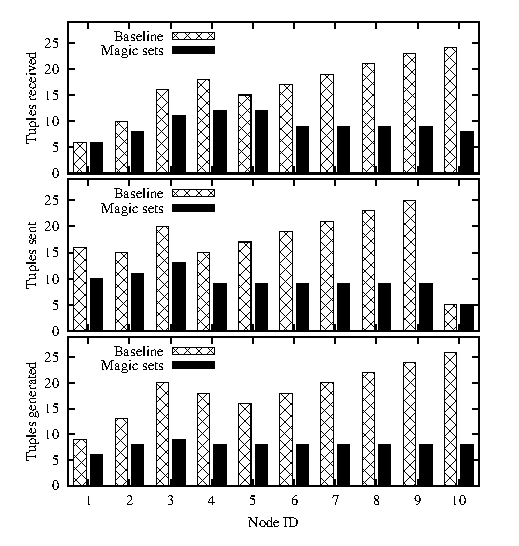
\includegraphics{figures/magicNumbers}
\ssp
\caption{For each node (node ID on $x$ axis), number of tuples received
  (top), sent (middle), and locally generated (bottom) on the $y$ axis.}
\label{ch:evita:fig:magicresults}
\end{figure*}

Figure~\ref{ch:evita:fig:magicresults}(a) shows the number of tuples that each
node receives from the network.  The magic-sets rewritten program causes no
more tuples to be received than the original, and for most nodes significantly
fewer when moving to nodes farther away from the clique.  That is because many
paths that are generated in the original program with destinations within the
clique other than node $1$ are pruned early on and never transmitted all the
way to the far end.  Similarly, Figure~\ref{ch:evita:fig:magicresults}(b) shows
the number of tuples each node transmits.  Again, the magic-rewritten program
does a lot better.  The two programs have similar tuple transmit/receive
overheads for nodes represents the number of tuples a node sends out over the
network.  The inclusion of the magic-sets rewrite reduces the number of sends
in all but one case (node $10$).  The node with identifier $10$ is the only
node with no incoming links and is therefore never burdened with network
traffic other than its own; as a result, though its received tuple overhead
benefits from magic sets, it transmitted tuple overhead is unaffected, since it
already sends out no extraneous paths other than its sole path towards node
$1$.  Finally, tuple storage is impacted beneficially by magic sets everywhere
(Figure~\ref{ch:evita:fig:magicresults}(c)), since both \ol{path} tuples
received from the network, and those generated locally for local consumption
are pruned away by the rewrite.



\section{Summary}
\label{ch:evita:sec:summary}


